\documentclass[11pt]{article}
\usepackage[T1]{fontenc}
\usepackage{lmodern}
\usepackage[margin=0.95in]{geometry}
\usepackage{amsmath,amssymb}
\usepackage{microtype}
\usepackage{enumitem}
\usepackage{xcolor}
\usepackage{tikz}
\usepackage[colorlinks=true,linkcolor=blue!50!black]{hyperref}

\newcommand{\C}{\mathbb{C}}
\newcommand{\abs}[1]{\lvert #1\rvert}
\newcommand{\norm}[1]{\lVert #1\rVert}
\newcommand{\key}[1]{\par\medskip\noindent{\normalsize\bfseries #1}\par\nobreak\vspace{-1pt}}
\setlist[enumerate]{leftmargin=1.5em,itemsep=3pt,topsep=3pt}

\title{\bfseries Step 4 of 5: two graphs and two cliques\\[5pt]
\large\normalfont Companion to \texttt{mub-outline.pdf}, Figure 1; preprint \S6}
\author{}
\date{}

\begin{document}
\maketitle
\vspace{-2.6em}

\noindent
\textbf{What this step receives.} For each seed ball and each certified region inside it, a closed set
of matrices known to contain every completion that the seed can produce.

\par\medskip\noindent\textbf{What it must produce.} A proof that no two further bases are unbiased to the first two
and to each other --- and, since the first two range over all seeds, a proof that no fourth basis
exists.

\key{1.\ Reduce the last question to a question about vectors}

Inside one certified region the first two bases are not known exactly, only up to a small
displacement. Write them as the standard basis $e_1,\dots,e_6$ and the columns $h_1,\dots,h_6$ of
$H/\sqrt6$. A vector $w\in\C^6$ is \emph{candidate} if
\[
\abs{\langle e_i,w\rangle}^2=\abs{\langle h_j,w\rangle}^2=\tfrac16
\qquad\text{for all } i,j ,
\]
that is, if it is unbiased to both bases. A third basis is six mutually orthogonal candidates; a
fourth is six more, orthogonal among themselves, unbiased to the first two bases, and unbiased to the
third --- thirty-six further scalar conditions.

\key{2.\ Cover the candidates, and keep the cover finite}

Candidate vectors again live in a torus of phases: bin the $36$ entrywise phases, then replace each bin
by a small Euclidean ball around a computed candidate. The output is a finite list of \emph{vector
balls}, each of which is either known to contain no candidate or merely not yet refuted. Note the
familiar shape: a cut, then balls inside the cut, exactly as in Step 1, one level down.

\key{3.\ Two necessary-condition graphs}

Make the vector balls the vertices of two graphs:
\[
O:\ \text{there is a possible orthogonal pair }(u,v),\qquad
U:\ \text{there is a possible unbiased pair }(u,v).
\]
An edge is retained whenever the corresponding condition has not been refuted, so $O$ and $U$ are
\emph{supersets} of the true orthogonality and unbiasedness relations. This is the crucial
orientation: the graphs are allowed to be wrong in one direction only.

\key{4.\ The pattern that a fourth basis would produce}

\begin{center}
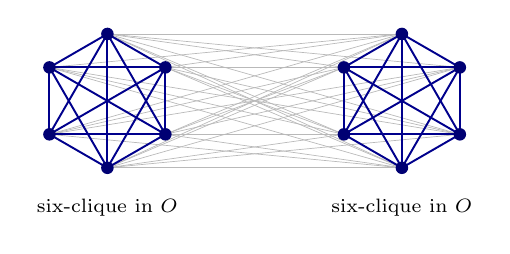
\begin{tikzpicture}[font=\small,dot/.style={circle,fill=blue!45!black,inner sep=1.6pt},scale=0.85]
\foreach \k/\dx in {L/0,R/4.4}{
  \coordinate (\k1) at (\dx+0,1); \coordinate (\k2) at (\dx-0.866,0.5);
  \coordinate (\k3) at (\dx-0.866,-0.5); \coordinate (\k4) at (\dx+0,-1);
  \coordinate (\k5) at (\dx+0.866,-0.5); \coordinate (\k6) at (\dx+0.866,0.5);}
\foreach \i in {1,...,6}{\foreach \j in {1,...,6}{\draw[gray!55,line width=0.25pt] (L\i)--(R\j);}}
\foreach \k in {L,R}{\foreach \i/\j in {1/2,1/3,1/4,1/5,1/6,2/3,2/4,2/5,2/6,3/4,3/5,3/6,4/5,4/6,5/6}{
    \draw[blue!55!black,line width=0.7pt] (\k\i)--(\k\j);}}
\foreach \k in {L,R}{\foreach \i in {1,...,6}{\node[dot] at (\k\i) {};}}
\node[align=center] at (0,-1.6) {\scriptsize six-clique in $O$};
\node[align=center] at (4.4,-1.6) {\scriptsize six-clique in $O$};
\end{tikzpicture}
\end{center}

\noindent
If two further bases exist, then $O$ contains two disjoint $6$-cliques --- the two bases --- and all
$36$ cross pairs are edges of $U$. The proof checks the contrapositive by finite enumeration: no
region produces that pattern, so no region produces the bases. Both directions of the implication are
worth fixing in mind. \emph{Absence} of the pattern is conclusive, because the graphs are larger than
reality. \emph{Presence} of the pattern proves nothing whatever.

\key{5.\ Why the obstruction is combinatorial and not analytic}

Single candidates are common. For the most symmetric pair of bases --- standard and Fourier --- Grassl
computed that exactly $48$ vectors are unbiased to both, forming $16$ bases none of which is unbiased
to another. So every local question has answers; what fails is the global assembly. Twelve vectors
must satisfy $15$ orthogonality conditions inside each basis and $36$ unbiasedness conditions across
them, and the last stage of the proof is a finite graph search rather than another estimate because the
obstruction lives in that pattern, not in a metric bound.

\key{Where this step can fail, and why that is safe}

Three failure modes, all benign. An edge test that is too weak leaves edges in the graphs, so the
forbidden pattern may appear in cases where it cannot occur in reality --- the search returns
``unresolved'', never a false exclusion. A graph too large to enumerate must be refined: more vector
balls, smaller ones. A bin that is too coarse must be split. As in Steps 1--3 the direction of the
implication is what keeps the argument sound, and the appendix's margins are what keep each edge test
honest.

\medskip
\noindent\textit{Note on sources.} The attached excerpt ends in \S3.3. This step is described from the
preprint's own \S1.2 summary of Stage C (phase-bin search, the $O$ and $U$ edges, two six-cliques with
all $36$ cross edges). The reader with the full text should consult \S6 for the edge tests themselves.

\end{document}
